\documentclass[minor, project]{gptcmdy}
\usepackage{tabularx}

\begin{document}

%
% Title page
%
%%%%%%%%%%%%

\title{This is your final project title for the report and presentation}
\author{Your Name}
\team{Member 2 (2301112346), Member 3 (2301112347), Member 4 (2301112348)}
\regno{2301112345}
\date{03-03-2026}
\acyear{2025-26}
\programme{Computer Engineering}
\department{Computer Engineering}
\maketitle

%%%%%%%%%%%%

\certificate

%%%%%%%%%%%%


% Acknowledgements
% Pleae change to express your gratitude

\acknowledgements

I express my sincere gratitude and thanks to \textbf{Mr. Biju M J}, Principal Govt. Polytechnic College, Mananthavady and \textbf{Mr. Karunakaran V N}, Head of the Computer Engineering Department for providing necessary facilities and their encouragement and support during the course of this project.

I owe special thanks to the project guide \textbf{Ms. Remitha N V}, Lecturer in Computer Engineering, \if@Project project \else\if@Seminar seminar \fi\fi coordinators \textbf{Mr. Amal Wilson}, Lecturer in Computer Engineering and \textbf{Ms. Aiswarya M}, Lecturer in Computer Engineering for their corrections, suggestions and sincere efforts to co-ordinate the project under a tight schedule.

I express my sincere thanks to all staff members in the Department of Computer Engineering who have taken sincere efforts in guiding and correcting me in conducting this project.

Next, I would like to acknowledge the heartfelt efforts, comments, criticisms,
co-operation and tremendous support given to me by my dear friends during the project
activities and also during the presentation without which this work would have been all the more difficult to accomplish.

Finally, I wish to thank my family and friends for their unwavering support and motivation, which kept me focused and driven to complete this report.
%%%%%%%%%%%%%%%%%%%%%%%%%%%%%%%

\begin {abstract}
Give a brief description of your work and its relevance in selected area of work. Try to keep the content in one or two paragraphs never exceeding a page.
\end{abstract}

\tableofcontents

\chapter{Introduction}

Give an overview of the topic in one or two paragraphs.

\section{Overview}
Brief summary of the project.

Lorem ipsum dolor sit amet, consectetur adipiscing elit. Etiam varius mauris massa, a sagittis purus vulputate et. Aenean egestas faucibus enim, non auctor nunc euismod quis. Sed finibus eget diam in dapibus. Nam lacinia ipsum sit amet libero cursus, vulputate tincidunt erat eleifend. Suspendisse malesuada neque in nibh laoreet, nec pulvinar urna maximus. Nullam faucibus urna a rutrum hendrerit. Pellentesque posuere ac quam ac ultrices. Cras aliquam dui quis ex mollis, a semper ex imperdiet. Nullam imperdiet vitae nunc a auctor. Duis sodales rutrum orci, at hendrerit erat tincidunt fermentum. In nec ornare nisi. Sed posuere urna suscipit ligula tristique, maximus imperdiet sapien sollicitudin. Vivamus ullamcorper elementum nisi, laoreet feugiat nisl.

Praesent commodo vestibulum odio, et elementum quam luctus vitae. Quisque pretium suscipit mauris sed auctor. Duis ullamcorper sed tortor ut commodo. Lorem ipsum dolor sit amet, consectetur adipiscing elit. Duis feugiat sapien vitae leo sodales finibus ac id felis. Sed pellentesque, mi ut lobortis vulputate, nisi magna fringilla urna, non tincidunt neque velit ac tellus. Duis fermentum tincidunt velit at porta. Nullam augue dolor, congue nec nisl vitae, placerat mollis dui. Nunc faucibus id lectus vitae vestibulum. Aliquam posuere quam vitae mi gravida, et efficitur diam mollis.


\section{Background \& Motivation}
Give reasons for the need of your project. Why this is needed, what was missing, what motivated you to do this project etc.

\section{Problem Statement}
State the problem here. Include what is missing, what are the problems due to that and son on, and what your project tries to solve.

\section{Objectives}
Clear, bulleted goals of your project work.
\begin{enumerate}
	\item Design a \dots
	\item Develop a \dots
	\item Optimize the \dots
\end{enumerate}

\section{Methodology}

A brief mention of the tools/approach used and why did you choose them.

\section{Organization of the Report}
Briefly explain how the report is organized like, Chapter 2 explains the objectives, Chapter 3 discusses about the objectives \dots.








\chapter{Requirements Specifications}

Specify the software requirement specifications

Lorem ipsum dolor sit amet, consectetur adipiscing elit. Etiam varius mauris massa, a sagittis purus vulputate et. Aenean egestas faucibus enim, non auctor nunc euismod quis. Sed finibus eget diam in dapibus. Nam lacinia ipsum sit amet libero cursus, vulputate tincidunt erat eleifend. Suspendisse malesuada neque in nibh laoreet, nec pulvinar urna maximus. Nullam faucibus urna a rutrum hendrerit. Pellentesque posuere ac quam ac ultrices. Cras aliquam dui quis ex mollis, a semper ex imperdiet. Nullam imperdiet vitae nunc a auctor. Duis sodales rutrum orci, at hendrerit erat tincidunt fermentum. In nec ornare nisi. Sed posuere urna suscipit ligula tristique, maximus imperdiet sapien sollicitudin. Vivamus ullamcorper elementum nisi, laoreet feugiat nisl.


\section{Methodology}
Specify the methods you used to collect and filter the requirements

\section{Hardware Requirements}
List of components (Microcontrollers, Sensors, Actuators).

\section{Software Requirements}
OS, IDEs (VS Code, Arduino IDE), Languages (C++, Python).

\section{Functional Requirements}
What the system must do.

\subsection{Requirement 1}
\subsection{Requirement 2}
\subsection{Requirement 3}

\section{Non Functional Requirements}
Reliability, power consumption, response time \dots

\subsection{Requirement 1}
\subsection{Requirement 2}
\subsection{Requirement 3}









\chapter{Design}

\section{System architecture}

\section{Circuit Diagram/Schematic}

\section{Dataflow Diagrams}

\section{Database Design}

\section{UI/UX Designs}


\chapter{Implementation}
\section{Module Descriptions and Interfaces}
Description of parts of your code.

\section{Core Algorithms}
Explaination of the logic.

\section{Challenges}
Technical challenges faced during the project


\chapter{Testing}
\section{Test Scenarios}
What are to be tested?

\section{Test Cases and Results}
A table showing test cases and their results.

\begin{tabularx}{\linewidth}{XXXXX}
\hline
No. & Input & Expected Result & Actual Result & Pass/Fail\\
\hline
\end{tabularx}

\section{Validation}
Does the project meet the original objectives?


\chapter{Results and Analysis}

\section{Screenshots}

This is how you will insert a figure. You can refer the figure like this. See Figure \ref{fig:exp1}.

\begin{figure}[!ht]
	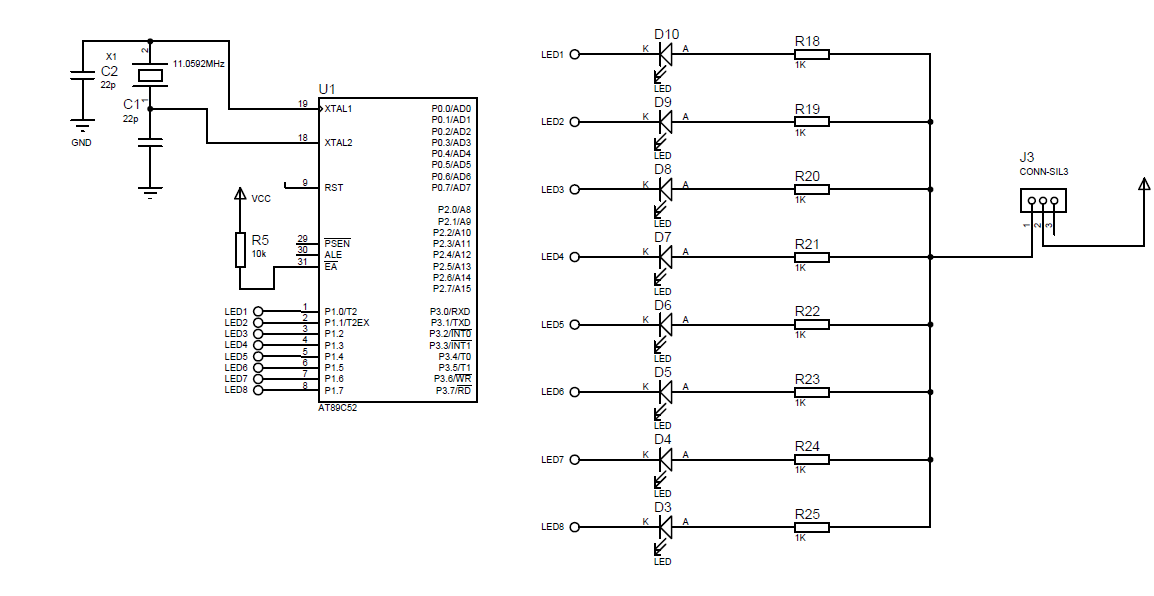
\includegraphics[width=\linewidth]{exp1}
	\caption{This is a sample figure}
	\label{fig:exp1}
\end{figure}

\section{Performance Analysis}
Response times, accuracy rates, or power efficiency.

\section{Comparison}
How your results compare to manual methods or existing tech.

\section{Limitations}
Honest look at what the system cannot do yet.

\chapter{Conclusions and Future Scope}
\section{Conclusion}
\section{Future Scope}

\bibliographystyle{ieeetr}
\nocite{*}
\bibliography{references}

\appendix
\chapter{User Manuals}
Specify the user manuals for your project, Installation steps, Operating instructions and Troubleshooting (Common errors and fixes).

\chapter{Datasheets of Components}
Summarized specs of the main sensors/IC.

\chapter{Source Code}
The entire source code. Preferrably provide the Github link to your project.
\end{document}

